\section{安装Kafka}

\subsection{简介}

Kafka是一种分布式队列工具,可以与Flume结合实现日志的收集和分发,也可以和Storm结合使用完成流式信息的处理。需要借助Zookeeper协调工作。

Kafka的作用和设置与Flume有很多相似的地方,下面可做一个对比。

\begin{itemize}
	\item Flume
		\begin{enumerate}
			\item 适合多个生产者
			\item 适合与Hadoop生态圈对接
			\item 适合下游消费者不多的情况
			\item 适合数据安全性不高的情况,如内存通道(Memory Channel)
		\end{enumerate}
	\item Kafka
		\begin{enumerate}
			\item 适合下游消费者众多的情况
			\item 适合在线的实时日志处理
			\item 适合数据安全性较高的情况
		\end{enumerate}
\end{itemize}

常见的一个模型是线上数据\(\rightarrow\)Flume\(\rightarrow\)Kafka\(\rightarrow\)Flume\(\rightarrow\)HDFS。

\subsection{配置文件}

Kafka有很多的配置可以添加,但是大部分保持默认即可,因此启动起来也很容易。启动简单的3个节点的集群需要配置的文件有:

\begin{itemize}
    \item \lstinline{server.properties},启动服务的基础配置,设置\lstinline{broker.id}和ZK集群信息。
    \item \lstinline{producer.properties},配置Producer信息。
    \item \lstinline{consumer.properties},配置Consumer信息。
    \item \lstinline{log4j.properties},配置日志输出信息。
\end{itemize}

Kafka使用了Zookeeper来做集群管理,在启动Kafka之前,要确保启动了ZK集群,如果没有配置ZK,也可以使用默认的
ZK服务,快速启动。
\begin{lstlisting}[style=mysh,title=快速启动Kafka]
# 启动自带ZK
$ bin/zookeeper-server-start.sh config/zookeeper.properties
# 然后启动Kafka
$ bin/kafka-server-start.sh config/server.properties
# 创建一个Topic
$ bin/kafka-topics.sh --create --bootstrap-server localhost:9092 --replication-factor 1 --partitions 1 --topic test
# 查看Topic
$ bin/kafka-topics.sh --list --bootstrap-server localhost:9092
test
# 现在可以发送一些信息
$ bin/kafka-console-producer.sh --broker-list localhost:9092 --topic test
This is a message
This is another message
# 新建一个窗口接受(消费)信息
$ bin/kafka-console-consumer.sh --bootstrap-server localhost:9092 --topic test --from-beginning
This is a message
This is another message
\end{lstlisting}

上面的例子就启动了一个单节点的单Broker的Kafka进程,并通过了简单的生产者消费者实验测试。
在Kafka中,也可以启动多个Broker的集群,

\begin{lstlisting}[style=mysh]
$ cp config/server.properties config/server-1.properties
$ cp config/server.properties config/server-2.properties
\end{lstlisting}

在下面两个文件中写入下面信息:

\begin{lstlisting}[style=mysh,title=config/server-1.properties]
broker.id=1
listeners=PLAINTEXT://:9093
log.dirs=/tmp/kafka-logs-1
\end{lstlisting}

\begin{lstlisting}[style=mysh,title=config/server-2.properties]
broker.id=2
listeners=PLAINTEXT://:9093
log.dirs=/tmp/kafka-logs-2
\end{lstlisting}

上面配置中的\lstinline{broker.id}要不同,由于是在单台机器上测试,因此这里设置了不同的监听端口
号和日志输出目录,防止各个broker覆盖各自的数据。

启动它们:

\begin{lstlisting}[style=mysh,title=启动多Broker集群]
$ bin/kafka-server-start.sh config/server-1.properties &
...
$ bin/kafka-server-start.sh config/server-2.properties &
...
# 创建新的Topic
$ bin/kafka-topics.sh --create --bootstrap-server localhost:9092 --replication-factor 3 --partitions 1 --topic my-replicated-topic
\end{lstlisting}

由于有多个Broker,使用\lstinline{--describe}查看各个Broker在干什么。

\begin{lstlisting}[style=mysh]
$ bin/kafka-topics.sh --describe --bootstrap-server localhost:9092 --topic my-replicated-topic
Topic:my-replicated-topic   PartitionCount:1    ReplicationFactor:3 Configs:
	Topic: my-replicated-topic  Partition: 0    Leader: 1   Replicas: 1,2,0 Isr: 1,2,0
\end{lstlisting}

关于输出,第一行描述了所有的分区信息,这里的分区数是1,后面的每行描述了分区的详细信息,因此后面只有1行。
可以从缩进关系中看出区别。

下面测试在多台机器多个节点上使用Kafka,这时已经启动了ZK集群而不是用自带的。在下列文件中加入下面内容:

\begin{lstlisting}[style=mysh,title=server.properties]
# 注意这里每台机器要不一样
broker.id=0
port=9092
# 这里每台机器也要求是不一样的,要与配置ZK集群中相同
host.name=master
listeners=PLAINTEXT://:9092
log.dirs=/home/zhangyu/kafka/data
\end{lstlisting}

\begin{itemize}
    \item \lstinline{broker.id},表示区分Broker的ID,每台机器都要修改,要不一样。
    \item \lstinline{port},表示服务的端口。
    \item \lstinline{log.dirs},存放log日志的目录。需要提前创建。
\end{itemize}

\lstinline{producer.properties}和\lstinline{consumer.properties}文件可以写好之后
在启动时指定配置文件的方式,也不配置,可以在启动时直接在命令行输入参数。
后面演示的是后者。这样更灵活,但是略显繁琐。生产时应该通过前者来配置。

\subsection{测试和运用}

启动流程:

\lstinputlisting[style=mysh,title=start-kafka.sh]{docs/kafka/start-kafka.sh}

注意,将\lstinline{kafka}文件夹直接拷贝到不同机器上后,修改\lstinline{broker.id}
的值后,每台机器上都需要启动Kafka服务。启动之后就可以新建窗口,进行后面的测试了。

\begin{center}
    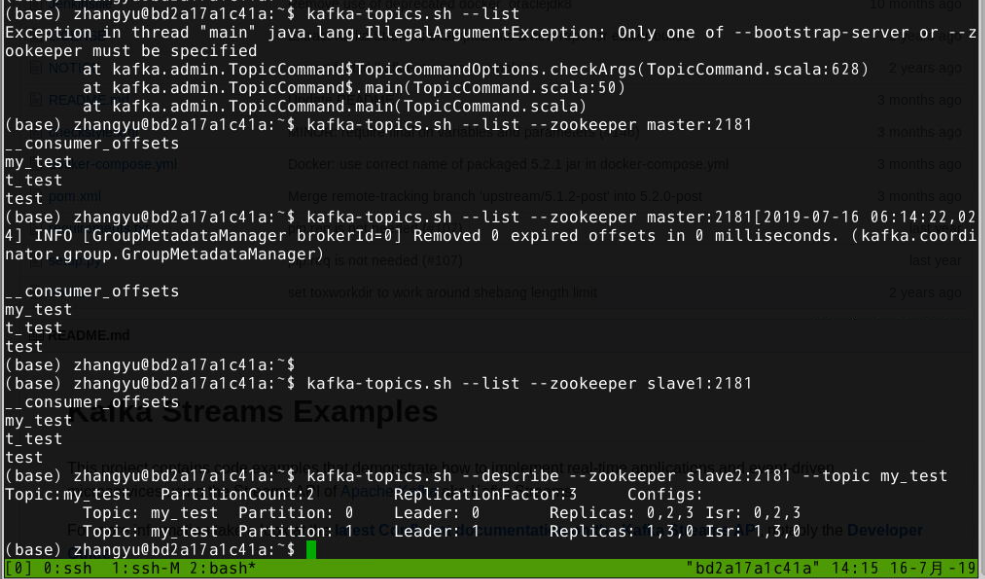
\includegraphics[width=\linewidth]{kafka/kafka-list.png}

    用\lstinline{kafka-topics --list}查看当前有的Topics。
\end{center}

\begin{center}
    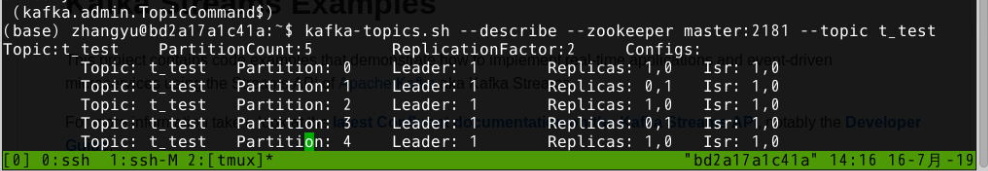
\includegraphics[width=\linewidth]{kafka/kafka-desc.png}

    用\lstinline{kafka-topics --describe}查看Topic的详细描述。
\end{center}

\begin{center}
    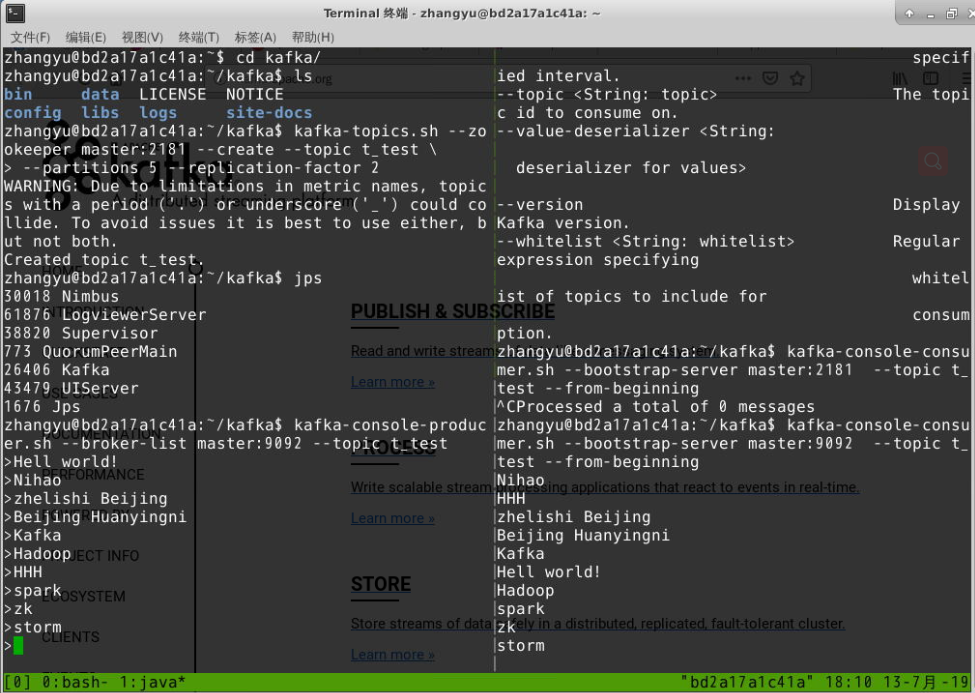
\includegraphics[width=\linewidth]{kafka/producomsu.png}

    可以看到左侧Producer产生出的数据直接就被右侧Consumer消费了。
\end{center}

\subsection{Java API实践}

Kafka提供了关于Consumer和Provider的高级API和低级API,使用高级API可以快速启动,但是灵活性较差,
而低级API比较灵活,应用较多,下面介绍高级API。
使用Kafka的Java API能够更加灵活地设置处理流程。

首先在Maven中加入依赖:
\begin{lstlisting}[style=myxml,title=pom文件中加入下面的依赖]
<dependency>
	<groupId>org.apache.kafka</groupId>
	<artifactId>kafka-clients</artifactId>
	<version>${kafka.version}</version>
</dependency>
\end{lstlisting}

\lstinline{kafka.version}中填入对应的Kafka版本。

然后编写调用Kafka关于生产者和消费者的API实现对应逻辑。

\lstinputlisting[style=customjava,title=CustomerProducer.java]{docs/kafka/CustomerProducer.java}

\lstinputlisting[style=customjava,title=CustomerConsumer.java]{docs/kafka/CustomerConsumer.java}

在测试的时候,需要在后台用命令行启动对应的Consumer或Provider进程,并且要有对应的Topic。

前面提到Flume与Kafka的对比和应用场景,下面是一个Flume与Kafka结合的配置书写。

\lstinputlisting[style=mysh,title=以Kafka作为Flume Sink的一个应用配置]{docs/kafka/flume-kafka.sh}
